We introduce Self-Reflective Retrieval-Augmented Generation (\model), shown in Figure~\ref{fig:taxonomy}. \model is a framework that enhances the quality and factuality of an LLM through retrieval and self-reflection, without sacrificing LLM's original creativity and versatility. 
Our end-to-end training lets an LM \mgen ~{\bf generate} text informed by {\bf retrieved} passages, if needed, and {\bf criticize} the output by learning to generate special tokens. 
These {\it reflection tokens} (Table~\ref{tab:reward}) signal the need for retrieval or confirm the output's relevance, support, or completeness. 
In contrast, common RAG approaches retrieve passages indiscriminately, without ensuring complete support from cited sources. 

\subsection{Problem Formalization and Overview}
\label{sec:overview}
Formally, given input $x$, we train \mgen to sequentially generate textual outputs $y$ consisting of multiple segments $y=[y_1, \dots, y_T]$, where $y_t$ indicates a sequence of tokens for the $t$-th segment.\footnote{
In this paper, we treat one sentence as a segment in our experiments, but our framework is applicable to any segment unit (i.e., sub-sentence).} 
Generated tokens in $y_t$ include text from the original vocabulary as well as the reflection tokens (Table~\ref{tab:reward}). 

\begin{table*}[t!]
\centering
\footnotesize
\begin{tabular}{p{2cm}p{1.2cm}p{3.5cm}p{5.5cm}}\toprule
Type & Input & Output & Definitions \\ \midrule
\ret   & $x$ / $x,y$ & \{yes, no, continue\} & Decides when to retrieve with \mret \\
\crel  & $x, d$  &\{{\bf relevant}, irrelevant\}  &   $d$ provides useful information to solve $x$. \\
\cgr  & $x, d, y$  &\{{\bf fully supported}, partially supported, no support\}  & All of the verification-worthy statement in $y$ is supported by $d$.   \\
\cuse & $x, y$  &\{{\bf 5}, 4, 3, 2, 1\}  & $y$ is a useful response to $x$.   \\
\bottomrule
\end{tabular}
    \caption{Four types of reflection tokens used in \model. Each type uses several tokens to represent its output values. 
    % \el{not sure whether this is correct?}. 
    The bottom three rows are three types of \crt~tokens, and {\bf the bold text} indicates the most desirable critique tokens. $x, y, d$ indicate input, output, and a relevant passage, respectively. 
    % \el{You use ``type'' in the table, which one should we use?}.
    }
    \label{tab:reward}
\end{table*}

\begin{algorithm}
\caption{\model Inference}\label{alg:self_reward inference}
\begin{algorithmic}[1]
\Require Generator LM \mgen, Retriever \mret, Large-scale passage collections $\{d_1, \ldots, d_N\}$ 
\State {\bf Input:} input prompt $x$ and preceding generation $y_{<t}$, {\bf Output:} next output segment $y_t$
\State \mgen predicts \ret~given $(x,y_{<t})$
\If{\ret~ == \texttt{Yes}}
    \State Retrieve relevant text passages $\mathbf{D}$  using \mret given $(x,y_{t-1})$ \Comment{\textcolor{blue}{Retrieve} }
    \State \mgen predicts \crel given $x, d$ and $y_{t}$ given $x,d, y_{<t}$ for each $d \in \mathbf{D}$ \Comment{\textcolor{blue}{Generate} }
    \State \mgen predicts \cgr and \cuse given $x, y_t, d$ for each $d \in \mathbf{D}$ \Comment{\textcolor{blue}{Critique} }
    \State Rank $y_t$ based on \crel, \cgr, \cuse \Comment{\textcolor{gray}{Detailed in Section~\ref{sec:fine_grained_decoding} }}
\ElsIf{\ret~ == \texttt{No}}
    \State $\mathcal{M}_{gen}$ predicts $y_t$ given $x$ \Comment{\textcolor{blue}{Generate} }
    \State $\mathcal{M}_{gen}$ predicts \cuse given $x,y_t$\Comment{\textcolor{blue}{Critique} }
\EndIf
\end{algorithmic}\label{algo:inference}
\end{algorithm}

\noindent {\bf Inference overview.}
Figure~\ref{fig:taxonomy} and Algorithm~\ref{algo:inference} present an overview of \model at inference. 
For every $x$ and preceding generation $y_{<t}$, the model decodes a retrieval token to evaluate the utility of retrieval. If retrieval is not required, the model predicts the next output segment, as it does in a standard LM.   
If retrieval is needed, the model generates: a critique token to evaluate the retrieved passage's relevance, the next response segment, and a critique token to evaluate if the information in the response segment is supported by the passage. Finally, a  new critique token evaluates the overall utility of the response.\footnote{We follow \citet{liu2023evaluating} in using a ``perceived'' utility value that is independent of retrieved passages.} 
To generate each segment, \model processes multiple passages in parallel and uses its own generated reflection tokens to enforce soft constraints (Section~\ref{sec:fine_grained_decoding}) or hard control (Algorithm~\ref{algo:inference}) over the generated task output. 
For instance, in Figure~\ref{fig:taxonomy} (right), the retrieved passages $d_1$ is selected at the first time step since $d_2$ does not provide direct evidence (\crel is {Irrelevant}) and $d_3$ output is only partially supported while $d_1$ are fully supported. 

\noindent {\bf Training overview.} 
% \textcolor{red}{Collecting fine-grained reflection tokens in scale is expensive~\cite{wu2023fine}. }
\model enables an arbitrary LM to generate text with reflection tokens by unifying them as next token predictions from the expanded model vocabulary (i.e., the original vocabulary plus reflection tokens). Specifically, we train the generator model \mgen on a curated corpus with interleaving passages retrieved by a {\it retriever} \mret and reflection tokens predicted by a {\it critic} model \mcrt (summarized in Appendix  Algorithm~\ref{alg:self_reward training}). We train \mcrt to generate reflection tokens for evaluating retrieved passages and the quality of a given task output (Section \ref{sec:critic_trainig}). 
Using the critic model, we update the training corpus by inserting reflection tokens into task outputs offline.  
Subsequently, we train the final generator model (\mgen) using the conventional LM objective (Section \ref{sec:gen_training}) to enable \mgen to generate reflection tokens by itself without relying on the critic at inference time. 

\subsection{\model Training}
Here,  we describe the supervised data collection and training of two models, the critic \mcrt 
(Section~\ref{sec:critic_trainig}) and the generator \mgen (Section~\ref{sec:gen_training}). 




\subsubsection{Training the Critic Model}
\label{sec:critic_trainig}

\noindent{\bf Data collection for critic model.} 
% (Line 3-6 in Algorithm \ref{alg:self_reward training}) 
Manual annotation of reflection tokens for each segment is expensive~\citep{wu2023fine}. 
A state-of-the-art LLM like GPT-4~\citep{openai2023gpt} can be effectively used to generate such feedback~\citep{liu2023gpteval}. 
However, depending on such proprietary LMs can raise API costs and diminish reproducibility%, as their behaviors change over time
~\citep{chen2023chatgpt}. 
We create supervised data by prompting GPT-4 to generate reflection tokens and then distill their knowledge into an in-house \mcrt. 
For each group of reflection tokens, we randomly sample instances from the original training data: $\{X^{sample}, Y^{sample}\} \sim \{X, Y\}$. 
{
As different reflection token groups have their own definitions and input, as shown in Table~\ref{tab:reward}, we use different instruction prompts for them. Here, we use \ret~ as an example. We prompt GPT-4 with a type-specific instruction (``Given an instruction, make a judgment on whether finding some external documents from the web helps to generate a better response.'') followed by few-shot demonstrations $I$ the original task input $x$ and output ${y}$ to predict an appropriate reflection token as text: $p(r|I, x, y)$.
Manual assessment reveals that GPT-4 reflection token predictions show high agreement with human evaluations.
We collect 4k-20k supervised training data for each type and combine them to form training data for \mcrt. 
Appendix Section~\ref{sec:instruction_gpt_4} shows the full list of instructions, and \ref{sec:data_collection_gpt4}} contains more details and our analysis.

\paragraph{Critic learning.}
% (Line 7 in Algorithm \ref{alg:self_reward training})
After we collect training data $\mathcal{D}_{critic}$, we initialize \mcrt with a pre-trained LM %parameterized by $\theta$ 
and train it on $\mathcal{D}_{critic}$ using a standard conditional language modeling objective, maximizing likelihood:
\begin{equation}\label{eq:crt_training}
    \max_{\mathcal{C}}\mathbb{E}_{((x,y),r) \sim \mathcal{D}_{critic}} \log p_{\mathcal{C}} (r| x, y), \text{ 
$r$ for reflection tokens. }
    % \el{does $r$ refer to the full set of tokens for a single response? } 
    % } r
\end{equation}
Though the initial model can be any pre-trained LM, we use the same one as the generator LM (i.e., Llama 2-7B; \citealt{touvron2023llama}) for \mcrt initialization. 
The critic achieves a higher than 90\% agreement with GPT-4-based predictions on most reflection token categories (Appendix Table~\ref{tab:reward_prediction}). 

\begin{figure}[t!]
  \begin{center}
    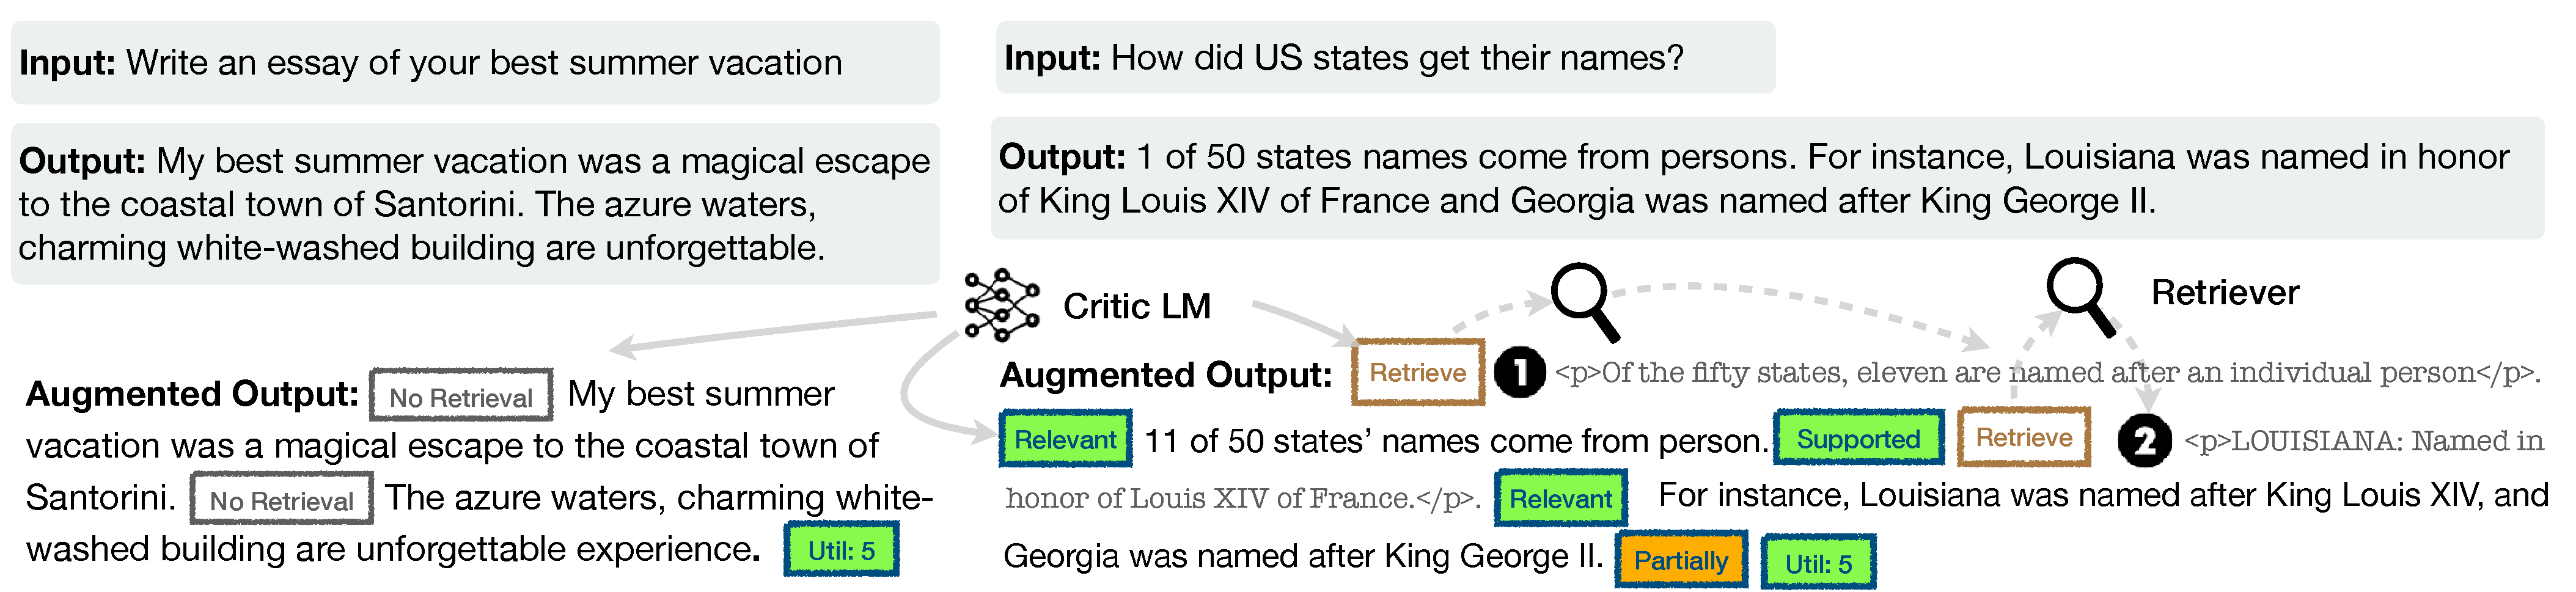
\includegraphics[width=0.95\textwidth]{figs/training_examples.pdf}
  \end{center}
  \caption{\model training examples. The left example does not require retrieval while the right one requires retrieval; thus, passages are inserted. More examples are in Appendix Table~\ref{tab:examplse_training_table}.}\label{fig:training_example}
\end{figure}

\subsubsection{Training the Generator Model}
\label{sec:gen_training}

\paragraph{Data collection for generator.}
Given an input-output pair $(x, y)$, we augment the original output $y$ using the retrieval and critic models to create supervised data that precisely mimics the \model inference-time process (Section~\ref{sec:overview}). 
For each segment $y_t \in y$, we run \mcrt to assess whether additional passages could help to enhance generation.  
If retrieval is required, the retrieval special token \ret~=\texttt{Yes} is added, and \mret retrieves the top $K$ passages, $\mathbf{D}$. 
For each passage, \mcrt further evaluates whether the passage is relevant and predicts \crel. 
% \hanna{all these tokens add a white space after which is weird.}
If a passage is relevant, \mcrt further evaluates whether the passage supports the model generation and predicts \cgr. 
Critique tokens \crel and \cgr are appended after the retrieved passage or generations.  
At the end of the output, $y$ (or $y_T$),  \mcrt predicts the overall utility token \cuse 
% \el{``IsComp'' sounds like measuring completeness instead of utility?}
, and an augmented output with reflection tokens and the original input pair is added to $\mathcal{D}_{gen}$. 
See the example training data in Figure~\ref{fig:training_example}. 




\noindent{\bf Generator learning.}
We train the generator model \mgen by training on the curated corpus augmented with reflection tokens $\mathcal{D}_{gen}$ using the standard next token objective:
\begin{equation}\label{eq:gen_training}
    \max_{\mathcal{M}}\mathbb{E}_{(x,y,r) \sim \mathcal{D}_{gen}} \log p_{\mathcal{M}} (y, r| x). 
\end{equation}
Unlike \mcrt training (Eq.~\ref{eq:crt_training}), \mgen learns to predict the target output as well as the reflection tokens.  
During training, we mask out the retrieved text chunks (surrounded by \texttt{<p>} and \texttt{</p>} in Figure~\ref{fig:training_example}) for loss calculation and 
expand the original vocabulary $\mathcal{V}$ with a set of reflection tokens $\{\crt, \ret\}$. 

\paragraph{Connections to prior work on learning with critique.}
Recent work 
%explicitly 
incorporates additional critique (feedback) during training, e.g.,  RLHF~(\citealt{ouyang2022training}) via PPO. 
While PPO relies on separate reward models during training, we compute critique offline and directly insert them into the training corpus, where the generator LM is trained with a standard LM objective. This significantly reduces training costs compared to PPO. 
Our work also relates to prior work that incorporates special tokens to control generation ~\citep{keskar2019ctrl,lu2022quark, korbak2023pretraining}. Our \model learns to generate special tokens {\it to evaluate its own prediction} after each generated segment,  
enabling the use of a soft re-ranking mechanism or hard constraints at inference (discussed next). 

\subsection{\model Inference}
\label{sec:fine_grained_decoding}
Generating reflection tokens to self-evaluate its own output makes \model controllable during the inference phase, enabling it to tailor its behavior to diverse task requirements. 
For tasks demanding factual accuracy~\citep{min2023factscore}, we aim for the model to retrieve passages more frequently to ensure that the output aligns closely with the available evidence. Conversely, in more open-ended tasks, like composing a personal experience essay, the emphasis shifts towards retrieving less and prioritizing the overall creativity or utility score. In this section, we describe approaches to enforce control to meet these distinct objectives during the inference process.

\noindent{\bf Adaptive retrieval with threshold.}
\model dynamically decides when to retrieve text passages by predicting \ret. 
Alternatively, our framework allows a threshold to be set. Specifically, if the probability of generating the {\ret=\texttt{Yes}} token normalized over all output tokens in \ret~ surpasses a designated threshold, we trigger retrieval (details in Appendix Section~\ref{sec:inference_details}).   


\noindent{\bf Tree-decoding with critique tokens.}
At each segment step $t$, when retrieval is required,  based either on hard or soft conditions, \mret retrieves $K$ passages, and the generator 
\mgen processes each passage in parallel and outputs $K$ different continuation candidates. 
We conduct a segment-level beam search (with the beam size=$B$) to obtain the top-$B$ segment continuations at each timestamp $t$, and return the best sequence at the end of generation. The score of each segment $y_t$ with respect to passage $d$ is updated with a critic score $\mathcal{S}$
% \el{We should change this, it has been used to mean retriever already; same for $t$ below that means both timestamp and token type} 
that is the linear weighted sum of the normalized probability of each \crt~token type. 
For each critique token group $G$ (e.g., \crel), we denote its score at timestamp $t$ as $s_t^G$, 
and we compute a segment score as follows:  
\begin{equation}
    f(y_t,  d, \crt) = p(y_{t} | x, d, y_{<t})) + \mathcal{S}(\crt){\rm , where}
\end{equation}
\begin{equation}\label{eq:reward}
    \mathcal{S}(\crt) = \sum_{G \in \mathcal{G}} w^G s_t^G %{\sum_{l} p(t_a^l) } 
    \mbox{ for } \mathcal{G} = \{\crel, \cgr, \cuse\}, 
\end{equation}
where  $s_t^G = \frac{p_t(\hat{r})}{\sum_{i=1}^{N^G} p_t(r_i)}$ stands for the generation probability of the most desirable reflection token $\hat{r}$ (e.g., \crel=\texttt{Relevant}) for the critique token type $G$ with $N^G$ distinct tokens (that represent different possible values for $G$). 
The weights $w^G$ in Eq.~\ref{eq:reward} are hyperparameters that can be adjusted at inference time to enable customized behaviors at test time. 
For instance, to ensure that result $y$ is mostly supported by evidence, we can set a weight term for the \cgr score higher, while relatively lowering weights for other aspects. 
Alternatively, we could further enforce hard constraints during decoding using \crt. 
Instead of using a soft reward function in Eq.~\ref{eq:reward}, we could explicitly filter out a segment continuation when the model generates an undesirable $\crt$ token (e.g., \cgr=\texttt{No support}) . 
% \el{to save space, we may be able to remove the following or at least shorten it? The content is mostly there in related work}
{Balancing the trade-off between multiple preferences has been studied in RLHF~\citep{touvron2023llama,wu2023fine}, which often requires training to change models' behaviors. \model tailors an LM with no additional training.  
}